\documentclass{article}

\usepackage{url}
\usepackage{epsfig}
\usepackage{graphicx}

\begin{document}

\title{eCryptfs v0.2 Design Document}

\author{Michael A. Halcrow}

\maketitle

\tableofcontents

\section{Introduction}

This document details the design for eCryptfs\footnote{To obtain
eCryptfs, visit \url{http://ecryptfs.sf.net}}. eCryptfs is a
POSIX-compliant enterprise-class stacked cryptographic filesystem for
Linux. It is derived from Erez Zadok's Cryptfs, implemented through
the FiST framework for generating stacked filesystems. eCryptfs stores
cryptographic metadata in the header of each file written, so that
encrypted files can be copied between hosts; the file will be
decryptable with the proper key, and there is no need to keep track of
any additional information aside from what is already in the encrypted
file itself.

eCryptfs is currently a native Linux filesystem included in the Linux
-mm tree (starting from 2.6.17). Mounting eCryptfs requires userspace
helper applications to perform some key management tasks; the
userspace components can be obtained from the eCryptfs project web
site.

The developers are implementing eCryptfs features on a staged
basis. The first stage (version 0.1) included mount-wide passphrase
support and data confidentiality enforcement. The second stage
(version 0.2) includes mount-wide public key support and data
integrity verification. The third stage (version 0.3) will include
per-file policy support. This document provides a technical
description of the eCryptfs filesystem release version 0.2.

Michael Halcrow has published two papers covering eCryptfs at the
Ottawa Linux Symposium (2004 and 2005)\footnote{See
\url{http://www.linuxsymposium.org/2006/proceedings.php}. The eCryptfs
paper is on page 209 of the first of the two halves of the proceedings
document.}. These papers provide a high-level overview of eCryptfs,
along with extensive discussion of various topics relating to
filesystem security in Linux.

\section{Threat Model}

eCryptfs protects data confidentiality in the event that an
unauthorized agent gains access to the data in a context that is
outside the control of a trusted host operating environment. Either a
secret passphrase or the private component of a public/private keypair
predicates access to the unencrypted contents of each individual file
object. An agent without the passphrase secret or private component of
the public/private keypair associated with any given file (see
Section~\ref{key_management}) should not be able to discern any
strategic information about the contents of any given encrypted file,
aside from what can be deduced from the file name, the file size, or
other metadata associated with the file. It should be about as
difficult to attack an encrypted eCryptfs file as it is to attack a
file encrypted by GnuPG (using the same cipher, key, etc.).

No intermediate state of the file on disk should be more easily
attacked than the final state of the file on disk. In the event of a
system error or power failure during an eCryptfs operation, no
partially written content should weaken the file's confidentiality,
and the file's integrity should still be verifiable. Attackers should
not be able to detect via a watermarking attack whether an eCryptfs
user is storing any particular plaintext. We assume that an attacker
potentially has access to every intermediate state of an encrypted
file on secondary storage.

eCryptfs offers no additional access control functions other than what
is already implementable via standard POSIX file permissions,
Mandatory Access Control mechanisms (i.e., SE Linux), and so forth.

eCryptfs provides data integrity verification in the event that an
unauthorized agent gains the ability to modify data in a context that
is outside the control of a trusted host operating environment. Once
the data has returned to a trusted host operating environment, the
user can verify that the file has not been modified by an agent that
does not possess at least one secret value necessary to access the
decrypted file contents. A user can also verify that a file's content
was generated by a particular individual with a given private key.

\section{Functional Overview}

eCryptfs is a stacked filesystem that is implemented natively in the
Linux kernel VFS. Since eCryptfs is stacked, it does not write
directly into a block device. Instead, it mounts on top of a directory
in a \emph{lower} filesystem. Most any POSIX-compliant filesystem can
act as a lower filesystem; EXT2, EXT3, and JFS are known to work with
eCryptfs. Objects in the eCryptfs filesystem, including \emph{inode},
\emph{dentry}, and \emph{file} objects, correlate in a one-to-one
basis with the objects in the lower filesystem.

eCryptfs is derived from Cryptfs\cite{cryptfs}, which is part of the
FiST framework developed and maintained by Erez Zadok\cite{fist}.

\subsection{VFS Objects}

eCryptfs maintains the reference between the objects in the eCryptfs
filesystem and the objects in the lower filesystem. The references to
the lower filesystem objects are maintained from eCryptfs via (1) the
file object's \emph{private\_data} pointer, (2) the inode object's
\emph{u.generic\_ip} pointer, (3) the dentry object's \emph{d\_fsdata}
pointer, and (4) the superblock object's \emph{s\_fs\_info}
pointer. The pointers for the eCryptfs dentry, file, and superblock
objects only reference the corresponding lower filesystem objects.

The inode \emph{u.generic\_ip} pointer references a data structure
that contains state information for cryptographic operations and a
reference to the lower inode object. The \emph{ecryptfs\_crypt\_stat}
structure is the inode cryptographic state structure; the contents of
this struct are given in Figure~\ref{comp_fig}. eCryptfs fills in the
\emph{ecryptfs\_crypt\_stat} struct from information stored in the
header region of the lower file (for existing files) or from the
mount-wide policy (for newly created files).

\subsection{VFS Operations}

\subsubsection{Mount}

At mount time, a helper application generates an authentication token
correlating either with a passphrase or with a public/prive keypair,
depending on options passed by the user. eCryptfs uses the keyring
support in the Linux kernel to store the authentication token in the
user's eCryptfs keyring. A mount parameter contains the identifier for
this authentication token. eCryptfs retrieves the authentication token
from the eCryptfs keyring using this identifier. It then uses the
contents of the authentication token to set up the cryptographic
context for newly created files. It also uses the contents of the
authentication token to access the contents of previously created
files.

\subsubsection{File Open}

The file format for the lower file is covered in this paper in
Section~\ref{file_format}.

When an existing file is opened
%\footnote{\emph{file.c::ecryptfs\_open()}}
in eCryptfs, eCryptfs opens the lower file and reads in the header. 
%\footnote{\emph{crypto.c::ecryptfs\_read\_headers()}}
The existence of an eCryptfs marker is verified, 
%\footnote{\emph{crypto.c::contains\_ecryptfs\_marker()}}
the flags are parsed, 
%\footnote{\emph{crypto.c::ecryptfs\_process\_flags()}}
and then the packet set is parsed.
%\footnote{\emph{keystore.c::ecryptfs\_parse\_packet\_set()}}

Each packet in the packet set is matched (via the identifier) against
an existing authentication token from the user's eCryptfs keyring. As
soon as eCryptfs finds a matching instantiated authentication token,
it uses that token to decrypt the encrypted file encryption key. If
the token is a passphrase token, eCryptfs generates the key that
encrypts the file encryption key via the S2K mechanism described in
Section~3.6 of RFC 2440\cite{rfc2440}. If the token is a public key
token, eCryptfs passes the encrypted file encryption key out to the
eCryptfs userspace daemon (See Section~\ref{kernel-daemon}), which
utilizes PKI subsystem to attempt to decrypt the file encryption
key. If eCryptfs cannot succeed in decrypting the encrypted file
encryption key, the open fails with a -EIO error code.

The header region may also contain root HMAC data packets and digital
signature packets. If an HMAC data packet is found, eCryptfs
associates the HMAC tree with the inode. If a digital signature packet
is found, eCryptfs verifies that signature against the root HMAC node
of the HMAC tree before continuing. If the signature cannot be
verified, eCryptfs returns -EIO on the open request.

eCryptfs generates a root initialization vector by taking the MD5 sum
of the file encryption key; the root IV is the first $N$ bytes of that
MD5 sum, where $N$ is the number of bytes constituting an
initialization vector for the cipher being used for the file.

While processing the header information, eCryptfs modifies the
\emph{ecryptfs\_crypt\_stat} struct associated with the eCryptfs inode
object.
%\footnote{\emph{(struct ecryptfs\_inode\_info *)(u.generic\_ip)$\rightarrow$crypt\_stat}}
The modifications to the \emph{ecryptfs\_crypt\_stat} structure
include:

\begin{itemize}
\item{Setting various flags, such as \emph{ECRYPTFS\_ENCRYPTED}.}
\item{Writing the inode file encryption key.}
\item{Writing the cipher name.}
\item{Writing the root initialization vector.}
\item{Writing the HMAC tree.}
\item{Filling in the array of authentication token signatures for the
  authentication tokens associated with the inode.}
\item{Setting the number of header pages.}
\end{itemize}

eCryptfs later uses this information when performing VFS operations.

When eCryptfs is opening a file that does not yet exist, it
initializes the \emph{ecryptfs\_crypt\_stat} structure according to
the mount-wide policy. eCryptfs uses this information to generate and
write the file header prior to any further VFS operations:

\begin{itemize}
\item{The file is encrypted.}
\item{The selected cipher.}
\item{The root IV is randomly generated.}
\item{The only authentication token associated with the file is the
  mount-wide passphrase or public keypair specified at mount time.}
\item{The HMAC tree and HMAC signature (if enabled at mount).}
\item{The header size, which is equal to the kernel's configured
  page size or 8192 bytes, which ever is greater.}
\end{itemize}

Once the \emph{ecryptfs\_crypt\_stat} structure is filled in, eCryptfs
initializes the kernel crypto API cryptographic context for the inode.
% \footnote{\emph{crypto.c::ecryptfs\_init\_crypt\_ctx()}}
By default, the cryptographic context is initialized in CBC mode and
is used in all subsequent page reads and writes.

\subsubsection{Page Read}

\label{page_read}

Reads can only occur on an open file, and a file can only be opened if
an applicable authentication token exists in the user's eCryptfs
keyring at the time that the VFS syscall that effectively opens the
file takes place.

On a page read, 
%\footnote{\emph{mmap.c::ecryptfs\_readpage()}}
the eCryptfs page index is interpolated into the corresponding lower
page index, taking into account the header pages and any HMAC pages
that may exist in the file (Section~\ref{file_format} details the
lower file format).
% \footnote{Release 0.1 ships with an experimental rotated/written IV
% mode of operation. The default (and recommended) mode of operation
% is derived IV mode, wherein no IV pages are written at all.}
eCryptfs derives the initialization vector for the given page index
%\footnote{\emph{crypto.c::ecryptfs\_derive\_iv()}}
by concatenating the ASCII text representation of the page offset to
the root initialization vector bytes for the inode and taking the MD5
sum of that string.

eCryptfs then reads in the encrypted page from the lower file and
decrypts the page. 
% \footnote{\emph{mmap.c::decrypt\_page()}}
eCryptfs first sets up the cryptographic structures to perform the
decryption.
% \footnote{\emph{crypto.c::do\_decrypt\_page\_offset()}}
It then makes the call to the kernel crypto API to perform the
decryption for the page.
% \footnote{\emph{crypto.c::do\_decrypt\_scatterlist()}}
This decrypted page is what gets returned via the VFS syscall to the
userspace application that made the request.

If the file header contained an HMAC data packet at the time that the
file was opened, eCryptfs verifies the HMAC for that page prior to
returning the data. If the calculated HMAC value does not match the
stored HMAC value, eCryptfs returns a -EIO from the VFS page read
call. Section~\ref{hmac} covers the HMAC processes in more detail.

\subsubsection{Page Write}

On a page write, 
% \footnote{mmap.c::ecryptfs\_writepage(); mmap.c::ecryptfs\_commit\_write}
eCryptfs performs a similar set of operations that occur on a page
read (see Section~\ref{page_read}), only the data is encrypted rather
than decrypted. The lower index is interpolated, the initialization
vector is derived, the page is encrypted with the file encryption key via the
kernel crypto API, and the encrypted page is written out to the lower
file.

If HMAC verification was enabled as a mount paramter, then... TODO

\subsubsection{File Truncation}

When a file is either truncated to a smaller size or extended to a
larger size, eCryptfs determines whether any truncation needs to occur
on the lower file; any truncation needed on the lower file will grow or
shrink the lower file by a multiple of an entire page. eCryptfs then
updates the filesize field (the first 8 bytes of the lower file) 
accordingly.

\subsubsection{File Close}

In eCryptfs releases through 0.2, eCryptfs never changes the
authentication packet set in the header after it initially creates the
file. When operating with HMAC verification enabled, eCryptfs
maintains two root HMAC value slots in the header.

When operating with HMAC verification enabled and when writing an
extent out to disk, eCryptfs first calculates all of the intermediate
HMAC values in the 2nd and 1st level HMAC extents, up to the new root
HMAC value. Before writing out the newly encrypted extent, eCryptfs
first writes out the new HMAC value into the least recently written
root HMAC slot. For efficiency reasons, eCryptfs may forestall writing
the 1st and 2nd level HMAC extents out to disk with the updated values
during regular data read/write operations until the file is closed.

When a file is no longer being accessed, the kernel VFS frees its
associated file, dentry, and inode objects according to the standard
resource deallocation process in the VFS.

\section{Cryptographic Properties}

\subsection{Key Management}

\label{key_management}

RFC~2440 (OpenPGP) heavily influences the design of eCryptfs, although
deviations from the RFC are necessary to support random access in a
filesystem. eCryptfs stores RFC~2440-compatible packets in the header
for each file. Valid packets include Tag 3 (passphrase) and Tag 11
(literal) pairs or Tag 1 (public key) and Tag 11 (literal) pairs. Each
file has a unique \emph{file encryption key} associated with it; the
file encryption key acts as a symmetric key to encrypt and decrypt the
file contents\footnote{Note that the \emph{file encryption key} is
analogous to the \emph{session key} referenced in RFC~2440}. eCryptfs
generates that file encryption key via the Linux kernel
\emph{get\_random\_bytes()} function call at the time that a file is
created. The length of the file encryption key is dependent upon the
cipher being used. By default, eCryptfs selects AES-128; the user can
select any cipher supported by the kernel crypto API.

Active eCryptfs inodes contain cryptographic contexts, with one unique
context per unique inode. This context exists in a data structure that
contains such things as the file encryption key, the cipher name, the root
initialization vector, signatures of authentication tokens associated
with the inode, various flags indicating inode cryptographic
properties, pointers to crypto API structs, and so forth. The
\emph{ecryptfs\_crypt\_stat} struct definition is in the
\emph{ecryptfs\_kernel.h} header file and is comprised of the elements
in Figure~\ref{comp_fig}.

\begin{figure*}[t]
  \begin{center}
    \begin{tabular}{|c|c|p{2in}|}
      \hline
      \emph{Name} & \emph{Type} & \emph{Description} \\
      \hline
      lock & Semaphore & Mutex for crypt stat object \\
      \hline
      root\_iv & Byte Array & The root initialization vector \\
      \hline
      iv & Byte Array & The current cached initialization vector \\
      \hline
      key & Byte Array & The file encryption key \\
      \hline
      cipher & Byte Array & Kernel crypto API cipher description
      string \\
      \hline
      keysig & Byte Array & Signature for authentication
      token associated with the inode \\
      \hline
      flags & Bit vector & Status flags (encrypted, etc.) \\
      \hline
      iv\_bytes & Integer & Length of IV \\
      \hline
      num\_header\_pages & Integer & Number of header pages for
      lower file \\
      \hline
      extent\_size & Integer & Number of bytes in an extent \\
      \hline
      key\_size\_bits & Integer & Length of file encryption key in
      bits \\
      \hline
      tfm & Crypto API Context & Bulk data crypto context \\
      \hline
      md5\_tfm & Crypto API Context & MD5 crypto context \\
      \hline
    \end{tabular}
    \caption{Contents of cryptographic stat structure (in kernel) for
    eCryptfs inode}
    \label{comp_fig}
  \end{center}
\end{figure*}

For each authentication token specified by the policy, the file encryption
key (as returned from \emph{get\_random\_bytes()}) is encrypted by the key
associated with the authentication token and stored in the first extent of
the \emph{lower} (encrypted) file. For releases 0.1 and 0.2 of eCryptfs
only one authentication token is supported: the mount-wide policy.
The key used to encrypt the file encryption key, that is the key
associated with the authentication token, is called the file key encryption
key.

The type of the authentication token indicates the encryption
mechanism for that key. eCryptfs 0.2 supports two types of authentication
tokens: passphrase authentication tokens (section \ref{passphrase_auth_tok}),
and public key authentication tokens (section \ref{pub_key_auth_tok}).
All authentication tokens are generated by the eCryptfs mount helper 
and inserted into the user's eCryptfs keyring
(a component of the Linux kernel keyring service), prior to mounting eCryptfs.

When eCryptfs opens an encrypted file, it attempts to match the
authentication token contained in the header of the file against the
instantiated authentication token for the mount point. If the
authentication token for the mount point matches the authentication
token in the header of the file, then it uses that instantiated
authentication token to decrypt the file encryption key that is used to
encrypt and decrypt the file contents on page write and read
operations.

\subsubsection{Passphrase Authentication Tokens}
\label{passphrase_auth_tok}

The file key encryption key associated with a passphrase authentication
token is the result of a conversion of the passphrase into a key.
This conversion follows the
S2K process as described in RFC~2440, in that the passphrase is
concatenated with a salt; that data block is then iteratively
MD5-hashed 65,536 times to generate the key that encrypts the file
encryption key. The signature for this type of token is the 16-byte
hexadecimal character representation of the first 8 bytes of the MD5 sum
of the file key encryption key.

\subsubsection{Public Key Authentication Tokens}
\label{pub_key_auth_tok}

Public key authentication tokens store the public key and a ``hint''
about the PKI where the key can be found. The public/private key pair
is used to encrypt and decrypt the file encryption key. The signature
for this type of token is the MD5 hash of the public key; the public
key is used to ensure that the authentication token (and therefore the
file) is not linked to a specific PKI. However, in order to facilitate
reasonable search times for the key pair, a hint is stored in the
authentication token about where the key was last known to be.

eCryptfs may have access to any number of Public Key Infrastructures
(PKI) via a pluggable module interface. Keys in individual PKI systems
generally have unique identifiers within those PKI systems. The
OpenSSL-specific key identifier is the path to a file on
disk containing an RSA public/private keypair. The GnuPG-specific key
identifier is the 8-digit hexadecimal key id.

\subsection{Cryptographic Confidentiality Enforcement}

eCryptfs enforces the confidentiality of the data that is outside the
control of the host operating environment by encrypting the contents
of the file objects containing the data. eCryptfs utilizes the Linux
kernel cryptographic API to perform the encryption and decryption of
the contents of its files over subregions known as \emph{extents}.

The length of each extent is fixed to 4096 bytes - eCryptfs requires
its host Linux kernel to be configured with its page size of at least
extent size; this ensures that a page is collection of extents. Each file
encrypted by eCryptfs contains a header with a size of either
the host kernel's page size, or of two extents (8192 bytes), which
ever is larger. This requirement for the header size being 8192
bytes at a minimum is to ensure page alignment when transitioning
a file between a 4k page size system and 8k page size system.

eCryptfs operates most efficiently when there is page alignment between
eCryptfs and the lower file system. Page alignment is the state where
a page of data in eCryptfs correlates a single page containing the
appropriate extents in the lower file system. Should page alignment
be disrupted, eCryptfs transparently maps the page indices and offsets
between the eCryptfs file and the lower file on read and write operations.

Each extent is independently encrypted. eCryptfs derives the
initialization vector (IV) for each extent from a \emph{root
initialization vector} that is unique for each file. eCryptfs offers
an HMAC verification policy option, which can be enabled via a mount
parameter. This enablement causes eCryptfs to associate the HMAC
verification policy with any new files that are created; if the option
is not enabled, HMAC verification is ignored. Files previously created
maintain their own policy, and are unaffected by this mount option.

eCryptfs calculates HMAC values over a fixed number $L$ of extents
and stores those values in headers preceeding the groups of extents; these
are the the 2nd level HMAC headers. eCryptfs also calculates HMAC values
over the 2nd level HMAC headers and stores them in the 1st level HMAC
headers. Finally, eCryptfs calculates a root HMAC value over all of
the 1st level HMAC extents and stores that root HMAC value in the
header. eCryptfs stores $x$ HMAC values per HMAC header, where
$x=\frac{HMAC header size}{HMAC value size}$. The HMAC header size is
the same as the eCryptfs header size, 8192 bytes or kernel page size, which
ever is larger. The 2nd level HMAC headers are
followed by $x * L$ extents of file data content; the set of all of the
2nd level HMAC headers followed by data extents for any given 1st
level HMAC header is known as an \emph{HMAC group}. The 1st level HMAC
header precede the first 2nd level HMAC header in each HMAC group.
Figure~\ref{hmac_file_format} illustrates the file format with HMAC
verification enabled.

\begin{figure*}[t]
  \begin{center}
    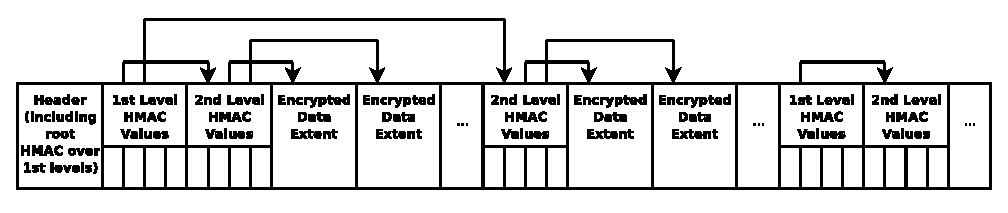
\includegraphics[width=0.75\textwidth]{file_format}
    \caption{File format with HMAC verification enabled.}
    \label{hmac_file_format}
  \end{center}
\end{figure*}

Figure~\ref{hmac_tree} gives a tree representation of the HMAC
structure.

\begin{figure*}[t]
  \begin{center}
    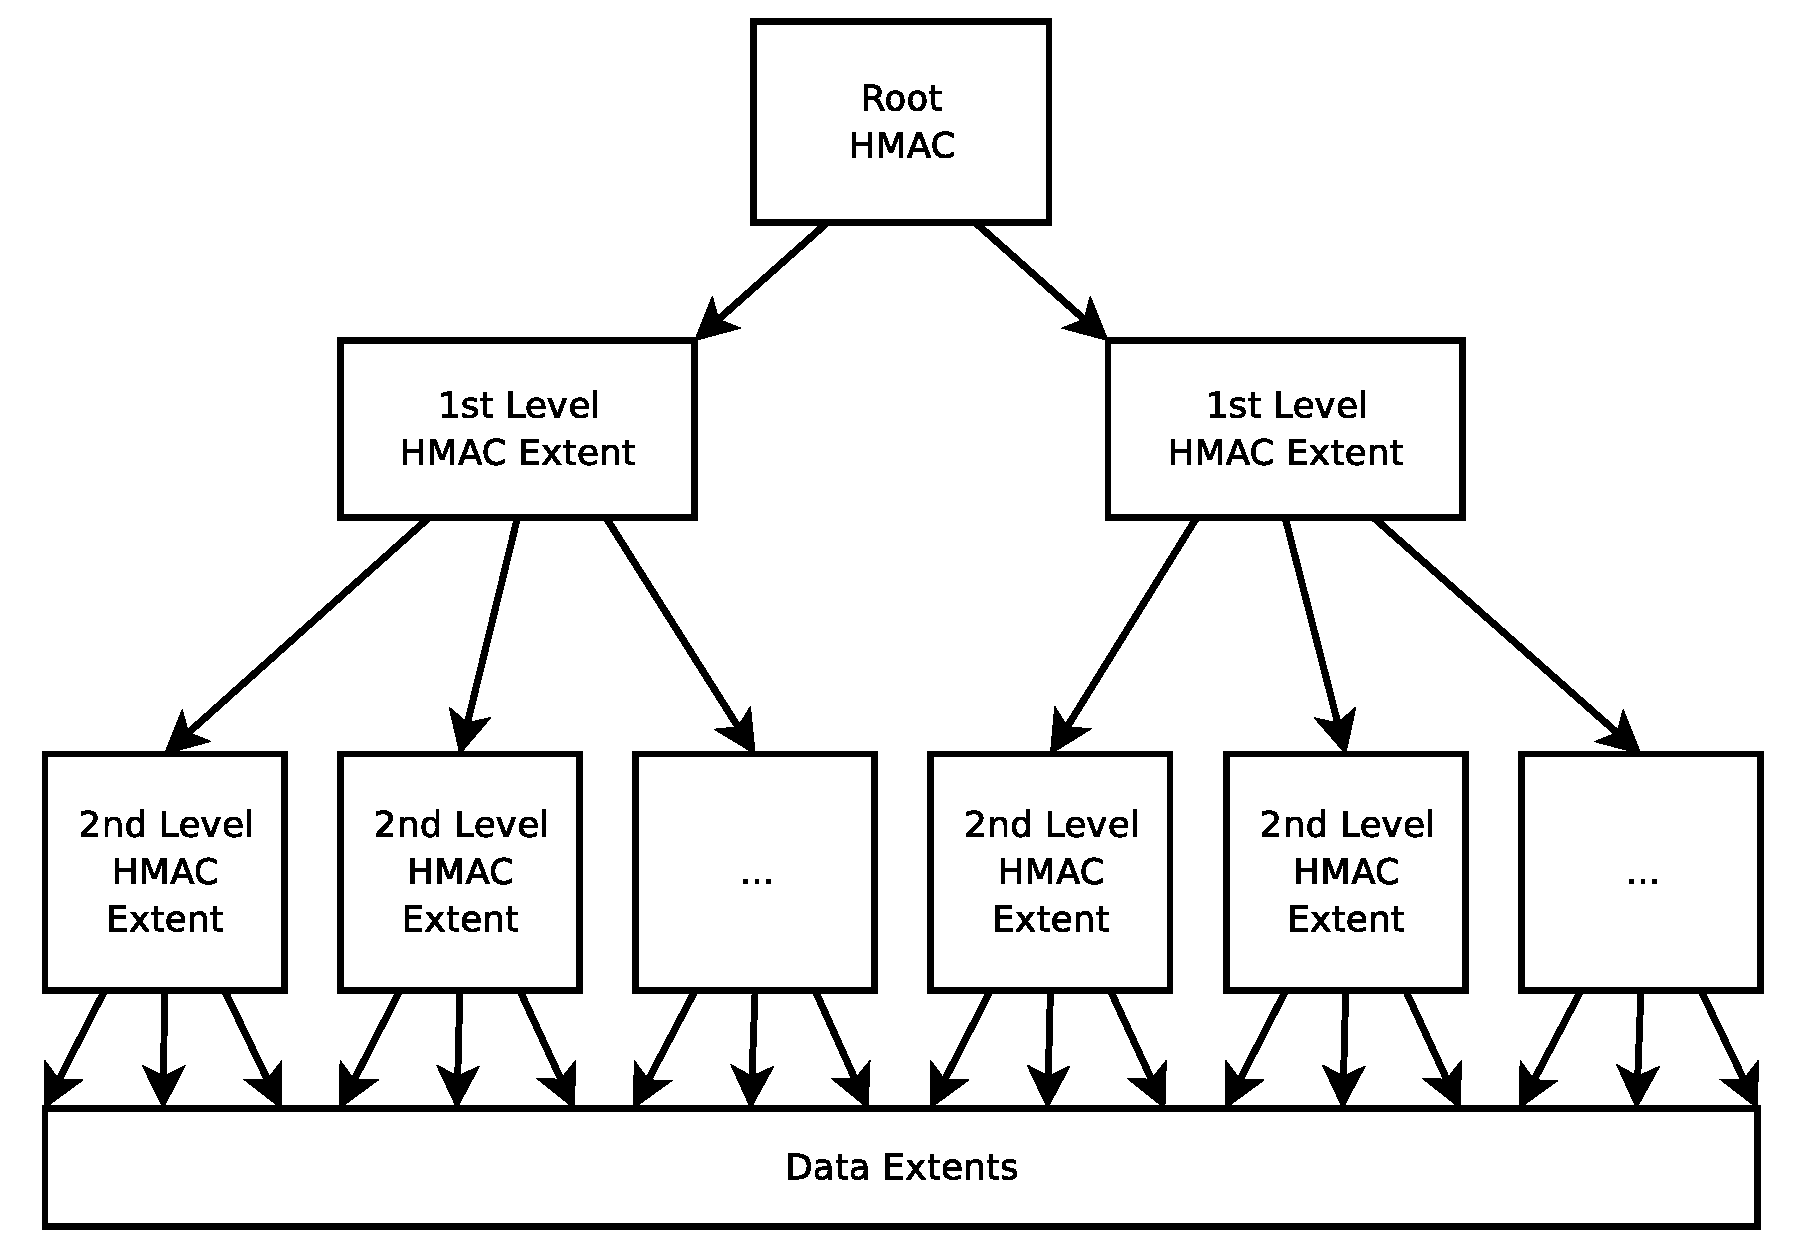
\includegraphics[width=0.85\textwidth]{hmac_tree}
    \caption{Simplified HMAC tree. Each 1st and 2nd level HMAC node
    contains one 4096-byte extent worth of HMAC values.}
    \label{hmac_tree}
  \end{center}
\end{figure*}

When a data extent is written, eCryptfs must update the appropriate
HMAC values in order to maintain consistency. On write, each HMAC node
lying on the path from the root HMAC to the 2nd level HMAC for the
modified extent must be regenerated. Figure~\ref{hmac_tree_update}
illustrates this operation.

\begin{figure*}[t]
  \begin{center}
    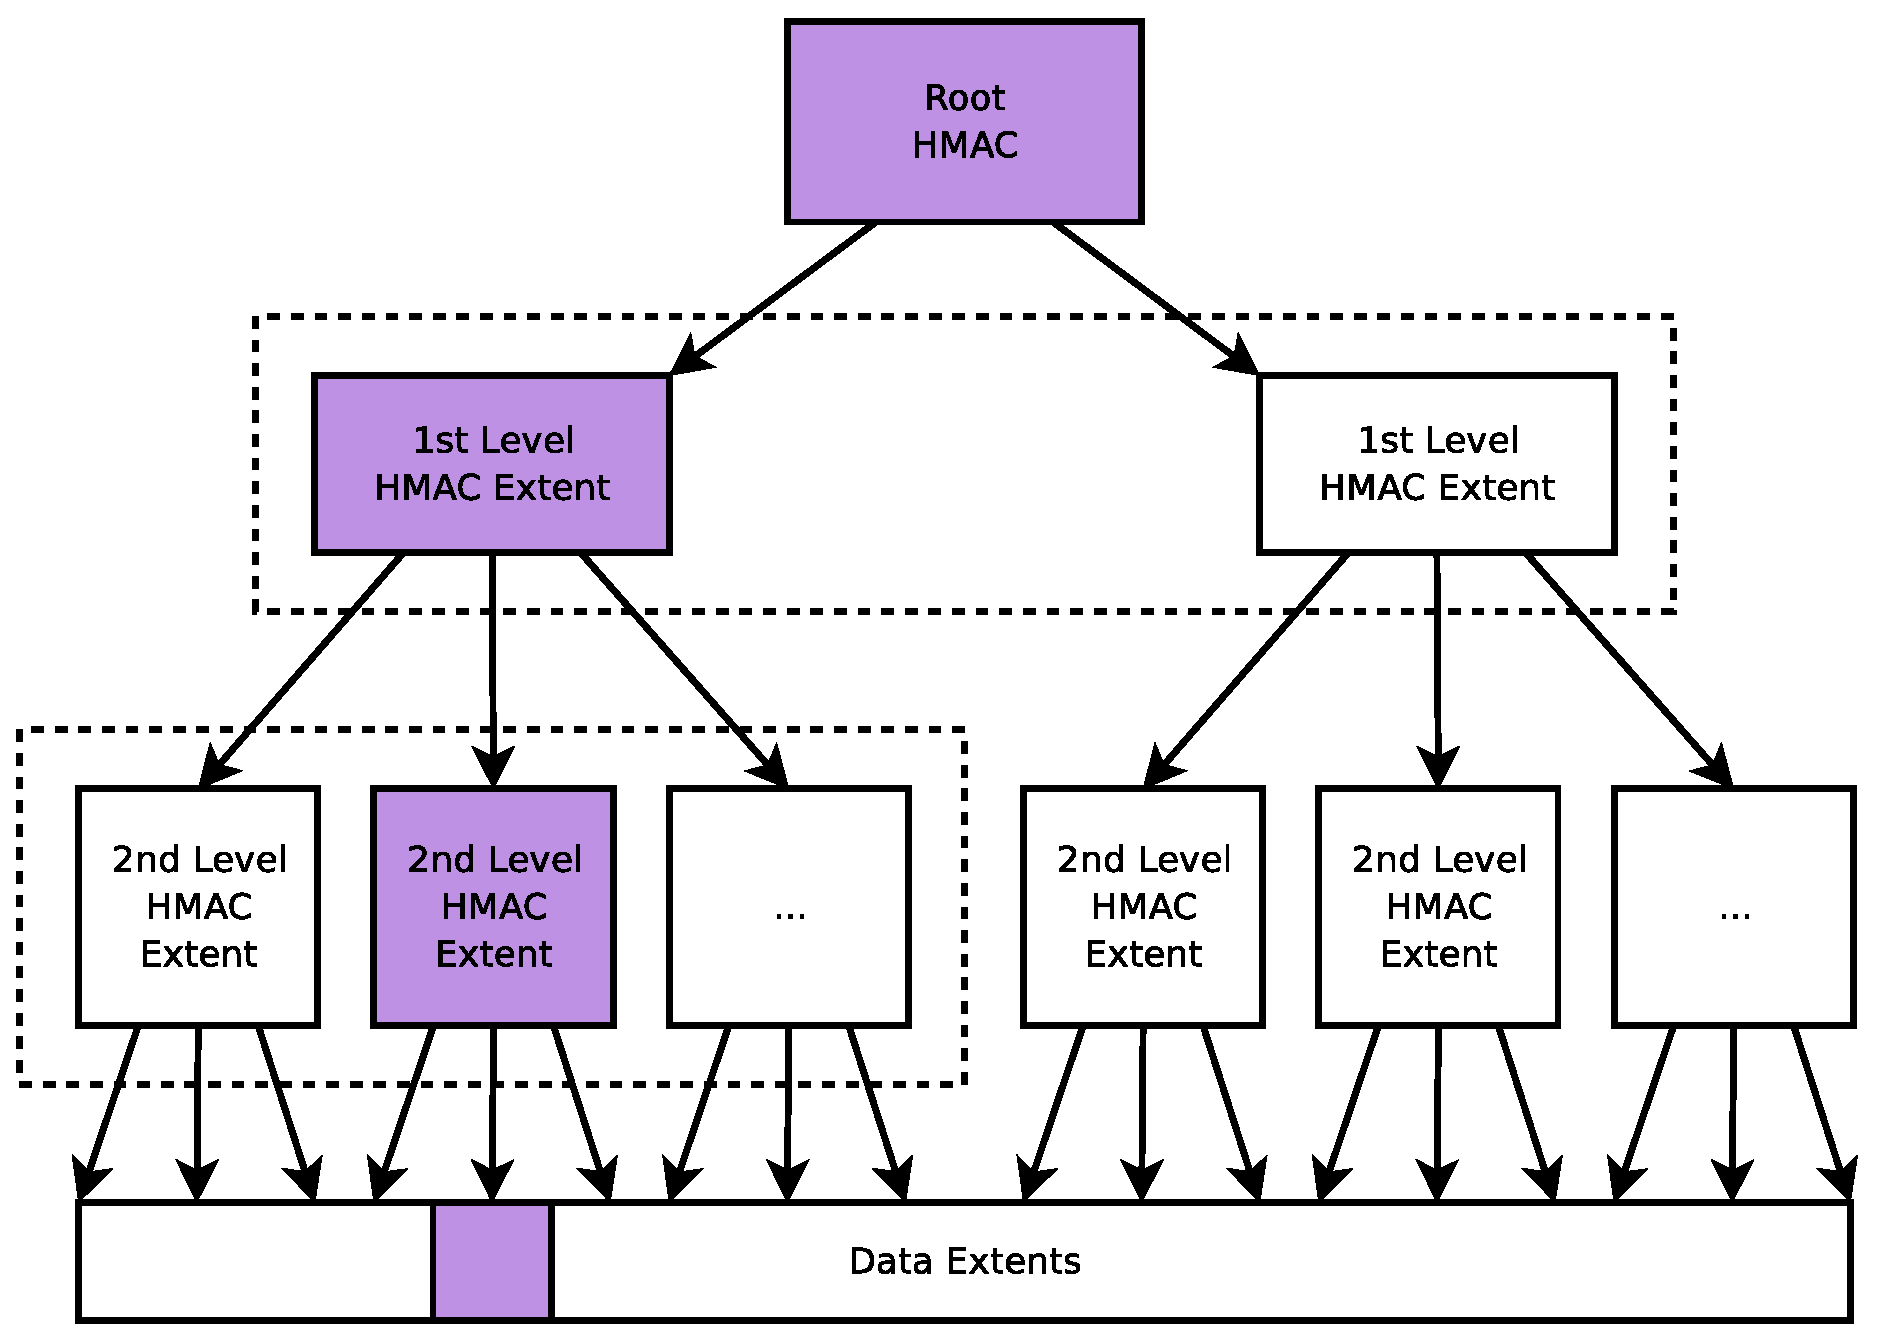
\includegraphics[width=0.92\textwidth]{hmac_tree_update}
    \caption{HMAC update. When a single data extent is modified,
    eCryptfs recalculates the corresponding HMAC value in the 2nd
    level HMAC extent. The 1st level HMAC extent covering that 2nd
    level HMAC extent is also recalculated. Finally, the root RHMC is
    recalculated across all of the 1st level HMAC extents. If HMAC
    values occupy 16 bytes each and if each 2nd level HMAC value
    covers a single data extent, then there will be one 1st level HMAC
    extent for every 256 megabytes of data in any given file.}
    \label{hmac_tree_update}
  \end{center}
\end{figure*}

When eCryptfs initially opens an eCryptfs file, it first validates all
of the 1st level HMAC extents in the file against the root HMAC value
in the header. On subsequent reads, eCryptfs validates each extent
against the corresponding HMAC value in the 2nd level HMAC extent, and
then eCryptfs validates the 2nd level HMAC extent against the
corresponding HMAC value in the previously-validated 1st level HMAC
extent.

\subsection{File Format}

\label{file_format}

The packet set consists of a combination of the following packets:

\begin{itemize}
\item{Tag 1 followed by either 1 or 2 Tag 11 identifiers}
\item{Tag 3 followed by a single Tag 11 identifier}
\item{Tag 11 containing HMAC data}
\item{Tag 2 containing digital signature on root HMAC}
\end{itemize}

The Tag 1 and Tag 3 packets store the encrypted file encryption key
and adhere to the specification given in RFC~2440. In release 0.2,
eCryptfs will only generate either a Tag 1 packet or a Tag 3 packet,
depending on the mount options. The Tag 11 root HMAC packet is
optional, based on a mount parameter to enable integrity
verification. A Tag 2 packet can only follow a Tag 11 root HMAC
packet. By default, Tag 2 packets are generated whenever Tag 11
packets are generated, unless explicitly disabled by a mount
parameter.

The first 26 bytes consist of the file size, the eCryptfs marker, a
set of status flags, and header extent size information. From byte 26
on, only RFC~2440-compliant packets are valid. All values more than
a single byte are written out in network byte order.

\scriptsize
\begin{verbatim}
Format version: 2

HMAC disabled:
  Header Extent:
    Octets 0-7:        Unencrypted file size
    Octets 8-15:       eCryptfs special marker
    Octets 16-19:      Flags
     Octet 16:         File format version number (between 0 and 255)
     Octets 17-18:     Reserved
     Octet 19:         Bit 1 (lsb): HMAC? (=0)
                       Bit 2: Encrypted?
                       Bits 3-8: Reserved
    Octets 20-23:      Header extent size
    Octets 24-25:      Number of header extents at front of file
    Octet 26:          Begin RFC 2440 authentication token packet set
    (Size is 8192 octets or page size of host one which file was
     created, whichever is greater)
  Data Extent 0:
    Lower data (CBC encrypted)
  Data Extent 1:
    Lower data (CBC encrypted)
  ...

HMAC enabled:
  Header Extent:
    As above; packet set includes Tag 11 root HMAC
  HMAC Level 1 Header [new HMAC group]
    Covers ((header extent size / HMAC value size) = N) HMAC Level 2 headers
  HMAC Level 2 Header
    Covers N*L Data extents, where L is the number of extents per HMAC value
  Data Extent 0:
    Lower data (CBC encrypted)
  Data Extent 1:
    Lower data (CBC encrypted)
  ...
  HMAC Level 2 Header
  Data Extent N*L
  Data Extent N*L+1
  ...
  HMAC Level 2 Header
  Data Extent 2N*L
  Data Extent 2N*L+1
  ...
  HMAC Level 1 Header [new HMAC group]
  HMAC Level 2 Header
  Data Extent N*N*L
  Data Extent N*N*L+1
  ...
\end{verbatim}
\normalsize

In the RFC~2440 packet set, each Tag 3 (passphrase) packet is immediately
followed by a Tag 11 (literal) packet containing the identifier for the
passphrase in the Tag 3 packet. This identifier is formed by hashing the
key that is generated from the passphrase in the String-to-Key (S2K)
operation.

Each Tag 1 (public key) packet is immediately followed by a Tag 11
(literal) packet containing the global key identifier. Optionally, one
additional Tag 11 packet containing a ``hint'' string may follow. The
format of the hint string is \emph{pki\_id:hint}, where \emph{pki\_id}
is a unique PKI module identifier and \emph{hint} contains a
suggestion to the PKI how the key may be found.

\subsubsection{Marker}

The eCryptfs marker for each file is formed by generating a 32-bit
random number ($X$) and writing it immediately after the 8-byte file
size at the head of the lower file. The hexadecimal
value\footnote{This value is arbitrary.} $0x3c81b7f5$ is XOR'd with
the random value ($Y=0x3c81b7f5\otimes X$), and the result is written
immediately after the random number.

\subsection{Kernel-userspace Communication Protocol}

\label{kernel-daemon}

The kernel code sends requests to the userspace code to perform public
key operations. The protocol for this communication is patterned after
RFC 2440 packets that are written to each file header (see Section~4
of RFC 2440).

\scriptsize
\begin{verbatim}
Public Key Decryption Request (tag 64)
  Content tag (64) (1 octet)
  Global key identifier size (1, 2, or 5 octets)
  Global key identifier
  Encrypted file encryption key size (1, 2, or 5 octets)
  Encrypted file encryption key

Public Key Decryption Reply (tag 65)
  Content tag (65) (1 octet)
  Status indicator: Zero on success, non-zero on error (1 octet)
  If status is zero:
    File encryption key size (1, 2, or 5 octets)
    File encryption key

Public Key Encryption Request (tag 66)
  Content tag (66) (1 octet)
  Global key identifier size (1, 2, or 5 octets)
  Global key identifier
  File encryption key size (1, 2, or 5 octets)
  File encryption key

Public Key Encryption Reply (tag 67)
  Content tag (67) (1 octet)
  Status indicator: Zero on success, non-zero on error (1 octet)
  If status is zero:
    Encrypted file encryption key size (1, 2, or 5 octets)
    Encrypted file encryption key
\end{verbatim}
\normalsize

The global key identifier is a string used as the ``signature'' of the
authentication token key object in the keyring. This authentication
token object contains additional information necessary for the
userspace code to complete the operation.

eCryptfs manages a netlink socket between the kernel module and the
userspace daemon. When the kernel would like to request a public key
operation from the userspace daemon on a file open event, the kernel
module allocates from a pool of free netlink message context
objects. It then constructs the request packet and sends it down to
the userspace daemon, after which the process calls the scheduler. The
daemon wakes up and parses the message, directing the request to the
appropriate PKI module. Once the request has been processed, the
daemon sends a reply packet via the netlink socket. A kernel thread
receives the reply, associates the received packet with its netlink
message context object, and wakes up the process that originally sent
the request out to userspace. The process parses the received packet
from the netlink message and continues with the file open operation.

\subsection{Deployment Considerations}

eCryptfs is concerned with protecting the confidentiality of data on
secondary storage that is outside the control of a trusted host
environment. eCryptfs operates on the VFS layer, and so it will not
encrypt data written to the swap secondary storage. It is recommended
that the user employ dm-crypt\footnote{See
\url{http://www.saout.de/misc/dm-crypt/}} to encrypt the swap space on
a machine where sensitive data may be loaded into memory at some
point.

Selection of a passphrase should follow standard strong passphrase
practices. eCryptfs ships with various helper applications in the
misc/ directory; use whatever tools are convenient for you to generate
a strong passphrase string. The user should store the string in a
secure place and use that as the passphrase when prompted.

\subsection{Cryptographic Summary}

The key design components for eCryptfs release 0.2 are:

\begin{itemize}
\item{Header page contains plaintext file size, eCryptfs marker,
  version, flags, header metadata, and RFC~2440 packets.}
\item{Either a mount-wide passphrase authentication token or a
  mount-wide public key authentication token is stored in the user's
  eCryptfs keyring.}
\item{Each file has a unique randomly-generate file encryption
  key. The file encryption key is encrypted and stored in the file
  header as a Tag 3 packet or as a Tag 1 packet as defined by
  RFC~2440.}
\item{The passphrase authentication token identifier, which is stored
  in the Tag 11 packet following the Tag 3 packet, is formed by taking
  the hash of the key that encrypts the file encryption key. The
  public key authentication token identifier is the MD5 hash of the
  public component of the public/private keypair.}
  \begin{itemize}
  \item{When using a passphrase authentication token, the key that
    encrypts the file encryption key is generated according to the S2K
    mechanism described in RFC~2440.}
  \end{itemize}
\item{The public key authentication token identifier is the MD5 hash
  of the public exponent of the public/private keypair.}
\item{Data extents, 4096 bytes in length, are encrypted with the
  selected cipher (CBC mode by default).}
\item{Each file's root initialization vector is the MD5 sum of the
  file encryption key for the file.}
\item{The initialization vector for each extent is generated by
  concatenating the root IV and the ASCII representation of the extent
  index and taking the MD5 sum of that string.}
\end{itemize}

\begin{thebibliography}{1}

\bibitem{rfc2440} J.~Callas, L.~Donnerhacke, H.~Finney, R.~Thayer,
``OpenPGP Message Format,'' RFC 2440, Internet Engineering Task Force,
Network Working Group, Nov. 1998,
\url{http://www.ietf.org/rfc/rfc2440.txt}; accessed March 13, 2006.

\bibitem{cryptfs} E. Zadok, I. Badulescu, and A. Shender. Cryptfs: A
Stackable Vnode Level Encryption File System. Technical Report
CUCS-021-98. Computer Science Department, Columbia University, 1998.

\bibitem{fist} E. Zadok and J. Nieh. FiST: A Language for Stackable
File Systems. To appear in USENIX Conf. Proc., June 2000.

\end{thebibliography}

\end{document}
